\documentclass[12pt, letterpaper, twoside]{article}
\usepackage{parskip}
\usepackage[utf8]{inputenc}
\usepackage{graphicx}
\usepackage{hyperref}
\graphicspath{ {images/} }

\title{Getting Comfy in the Command Line}
\author{Can221-ParOS \thanks{Huge thanks to \href{https://www.youtube.com/channel/UC2eYFnH61tmytImy1mTYvhA}{Luke Smith}, \href{https://www.youtube.com/channel/UCVls1GmFKf6WlTraIb_IaJg}{DistroTube}, and \href{https://www.youtube.com/channel/UC7YOGHUfC1Tb6E4pudI9STA}{Mental Outlaw}. They are where I gained my immense interest in Linux.}}
\date{August 14, 2020}

\begin{document}
\maketitle


Using the information in this document, you should be able to quickly learn how to use a Linux system to its full potential, and in the process become more proficient and comfortable in the Command Line (Commonly referred to as the Terminal). If you want to skip the fluff and get into the information, the next page is where it starts. This page is just an introduction and some eye candy. 


In figure \ref{figure:image1} below I show my desktop, with two different terminals open. 

One is only open as a prompt inside a folder, and the one below it has the vim text editor open, editing a \LaTeX{} document file. 
In fact, this PDF was originally written as a \LaTeX{} document using vim.


\begin{figure} [ht]
        \centering
	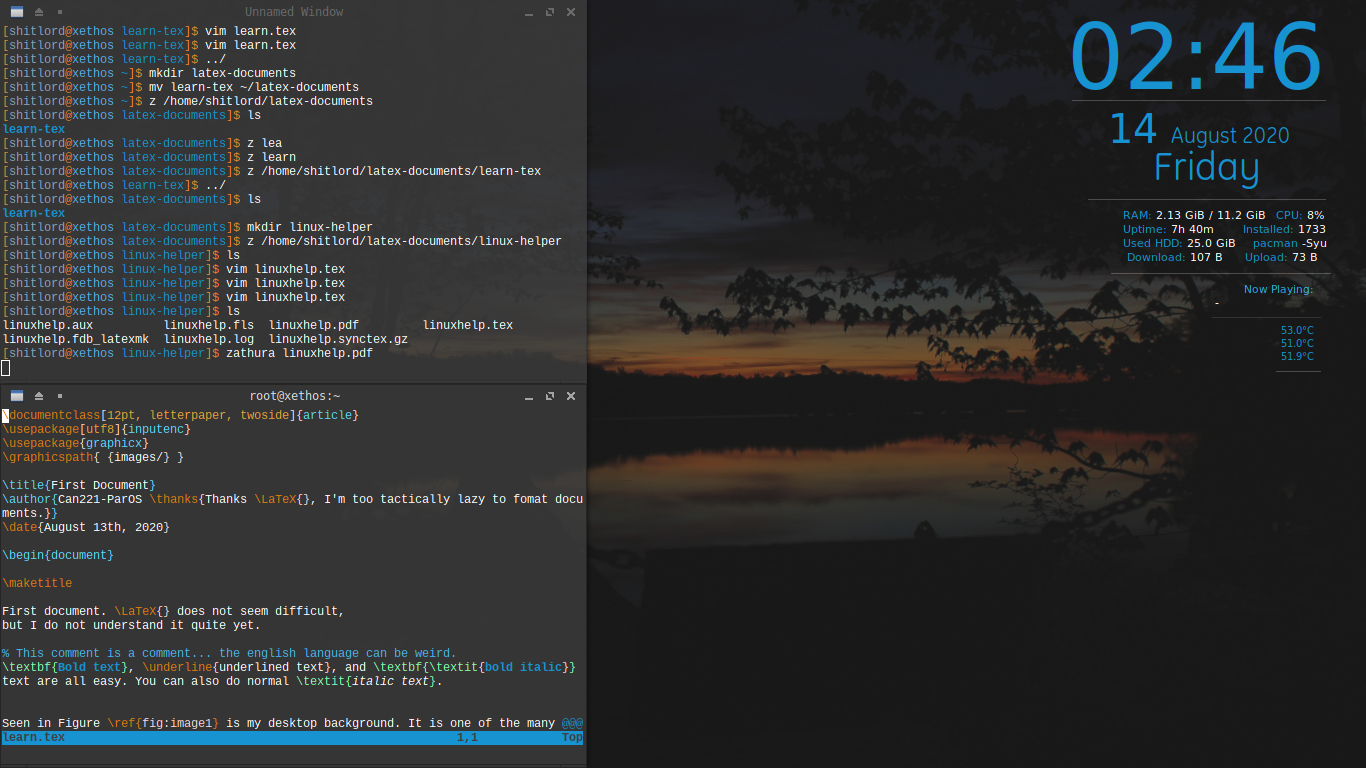
\includegraphics[width=0.60\textwidth]{screen}
	\caption{Two open terminals}
	\label{figure:image1}
\end{figure}

\section{Navigation}


This section focuses on navigating through files in the Terminal. We will go over commands like cd, ls, and certain tricks to make navigation easier and faster.

\textbf{ls} : Lists the contents of the current directory (folder). It has many options you can pass it, but the most important is \textbf{ls -a}. This will list all of the files in the current directory, including ones that start with a dot/period

An example of \textbf{ls} can be seen in figure \ref{figure:image2}, at the end of this section.

\textbf{cd} : Changes the current directory. You can use the full path to a file using \textbf{cd /full/path}. If the file is in the $\mathtt{\sim}$/ folder, you can use \textbf{$\mathtt{\sim}$/folder}. If the file is inside of the current directory, you can also simply use \textbf{cd file}. cd also has very useful built in shortuts : \textbf{cd $\mathtt{\sim}$} will take you to your home directory, and \textbf{cd -} will take you right back into the last folder you cd'd into. 

An example of \textbf{cd} can also be seen below, in figure\ref{figure:image3}.

\textbf{file} : Tells you the type of file that you specify. Useful to help identify if a file is a directory, text, or an executable. For example, if I was in the Home directory and wanted to figure out was type of file Documents is I would use \textbf{file Documents}

As with the others, there is an example of the file command in use seen below, in figure \ref{figure:image4}.

\begin{figure}[!htb]
\minipage{0.32\textwidth}
  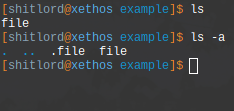
\includegraphics[width=0.88\textwidth]{listfile}
  \caption{List command}\label{figure:image2}
\endminipage\hfill
\minipage{0.32\textwidth}
  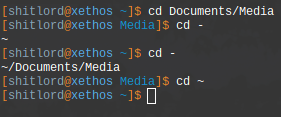
\includegraphics[width=0.88\textwidth]{cddemo}
  \caption{Cd command}\label{figure:image3}
\endminipage\hfill
\minipage{0.32\textwidth}%
  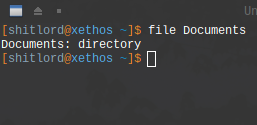
\includegraphics[width=0.88\textwidth]{filecmd}
  \caption{File command}\label{figure:image4}
\endminipage
\end{figure}


\newpage
\section{File Management}

This section will go over managing your files in linux, and the commands used to create and remove files, and the tricks that make it easier and faster.

\textbf{mkdir file} will create a directory named "file" in the current working directory. To make a file in a specified location, use the path to the desired file before the directory you want to make. For example, \textbf{mkdir $\mathtt{\sim}$/Documents/Media} will create a directory named "Media" inside the $\mathtt{\sim}$/Documents directory. An example can be seen in figure \ref{figure:mkdirex} below.

\textbf{rm file} deletes "file". To remove a directory, you need to use \textbf{rm -rf directory}. \textbf{\textit{Use rm carefully. It does not send files to the recycle bin, it deletes them immidiately.}}. The special character \textbf{*} can be used to delete all files in the current directory, \textbf{\textit{this is very useful, but also very dangerous.}} An example of \textbf{*} pattern matching to delete a specific group of files can be seen below in figure \ref{figure:rmpatex}. 

\begin{figure} [!htb]
\minipage{0.52\textwidth}
  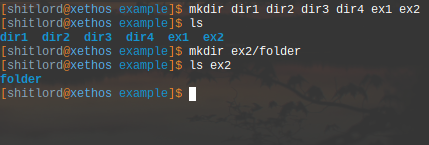
\includegraphics[width=0.88\textwidth]{mkdirex}
  \caption{Exaple of mkdir}\label{figure:mkdirex}
\endminipage\hfill
\minipage{0.48\textwidth}
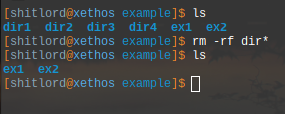
\includegraphics[width=0.88\textwidth]{rmpatex}
  \caption{Pattern matching with rm}\label{figure:rmpatex}
\endminipage
\end{figure}

\textbf{Linux Filestructure} - A brief explanation of the structure of the filesystem in linux. \textbf{/home/username or "$\mathtt{\sim}$/"} is where the user files are stored, and the user does not need to use sudo to modify these files. The files in the \textbf{/ or root} directory are system files, configuration defaults, and some application files. To modify files in the \textbf{/ or root} directory, you need to use sudo and enter your password, because those files are owned by the root account. This is one of the things that makes linux such a secure OS.

A great video about the Linux filesystem can be found here: 
(Double-click to open link)

\url{http://www.youtube.com/watch?v=HbgzrKJvDRw&t=4s}

\section{Package Management}

Package Management is one of the most important and powerful aspects of Linux Operating Systems. Package Managers allow you to manage \textit{all} of the software on your system, down to the linux kernel you are using. 

Arch based distros (Manjaro, Artix and others) are \textit{rolling release}. This means that as updates are released by the developers, they are available to the user immediately (\textit{Somewhat immediately}, as manjaro and certain arch repositories hold back updates a few weeks for testing stability and patching bugs). It is best practice to update your system before installing new software, to ensure all the other things it relies on are up to date. I will go over only the pacman commands, as they are the same as the yay package manager commands.

\textbf{pacman -Syyu} this will sync your package mirrors to ensure they are up to date, and then update all packages on the system (including the kernel, and other OS packages. \textbf{pacman -S package-name} installs the package "package-name", if it exists. \textbf{pacman -R pacage-name} removes "package-name" if it is installed on the system. \textbf{pacman -Ss key words} searches the repository for packages related to "key words".

\textbf{pacman -Sy} \textbf{\textit{Do not use this command. It leaves your system in a partially upgraded state, which can break the system on the next update. Use }pacman -Syu or pacman -Syyu instead}

\begin{figure} [ht]
	\centering
	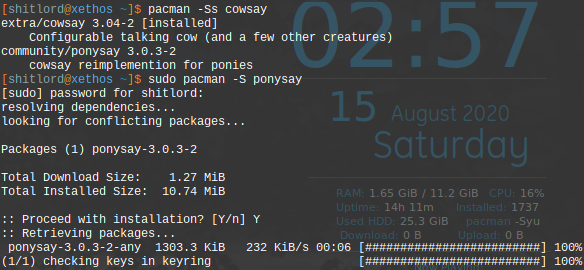
\includegraphics[width=0.75\textwidth]{pacman}
	\caption{Pacman package manager, searching and downloading a program}
\end{figure}

\newpage
\section{CLI Text Editors}

Chances are, you've been using a GUI text editor. This section will explain the basics of Command Line (CLI) text editors like Nano, and more specifically \textit{Vim/NeoVim}.

\textbf{nano} will open the Nano text editor in the terminal. Once opened, nano will look like the image seen at figure \ref{figure:nano}

\begin{figure} [ht]
	\centering
	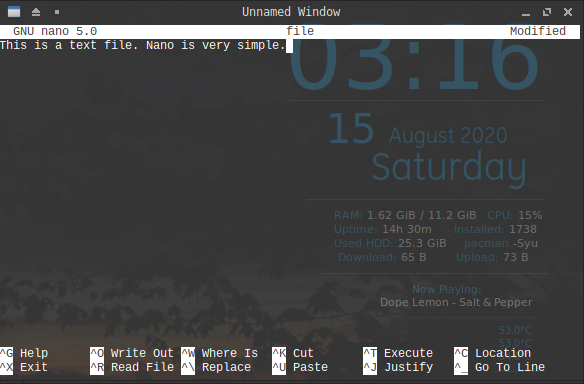
\includegraphics[width=0.70\textwidth]{nano}
	\caption{Nano text editor}
	\label{figure:nano}
\end{figure}

It looks a bit complicated at first, but all the keybindings are \textbf{Ctl} and the displayed letter. For example \textit{to save use \textbf{Ctl O}}, then press enter to confirm. It will also ask if you want to save when you exit, and you can press Y or N to save, or quit without saving. It works much the same for all the other functions. To move the cursor, simply use the arrow keys. Nano is easy enough, so it shouldn't take long to get used to.

\newpage
\textit{\textbf{Vim/NeoVim}}

Vim (which has been around since 1991!), or its more modern alternative, neovim is an extremely powerful text editor. Sadly though, it is most well known for people who dont know how to use it getting stuck in it, not knowing how to save or even exit the editor and get back to the command line. It has many different keystrokes and Vim commands that I am going to explain in detail, because they make editing text or writing certain programming languages seem like a form of black magic you are the master of.

When you open Vim/NeoVim, you will be in \textbf{NORMAL} mode, and vim wont let you type in text. \textbf{NORMAL} mode will only recognize vim's keybindings. You can enter \textbf{NORMAL} mode at any time by pressing escape (esc). \textbf{NORMAL} mode can be seen in figure \ref{figure:normalm}.

To write or remove text in vim like usual, you need to be in \textbf{INSERT} mode. To enter \textbf{INSERT} mode, press the \textbf{i} key. Vim should now look like figure \ref{figure:insertm}, and you will be able to write text, and remove it with backspace.


\begin{figure} [!htb]
\minipage{0.45\textwidth}
  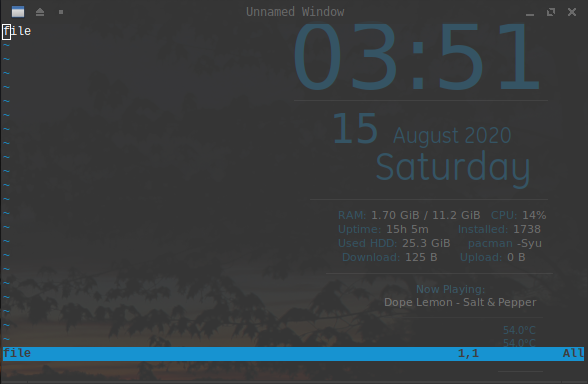
\includegraphics[width=0.88\textwidth]{normalm}
  \caption{Vim normal mode}\label{figure:normalm}
\endminipage\hfill
\minipage{0.45\textwidth}%
  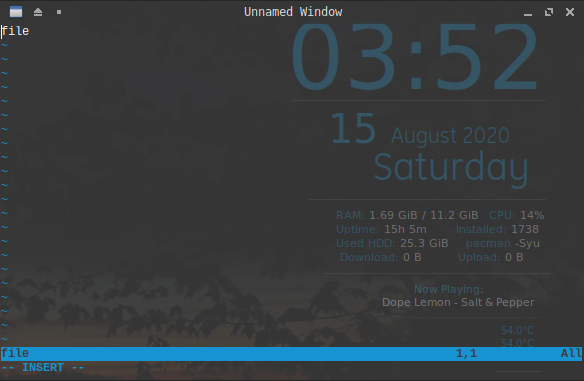
\includegraphics[width=0.88\textwidth]{insertm}
  \caption{Vim insert mode}\label{figure:insertm}
\endminipage
\end{figure}


\textbf{Normal mode keybindings} - \textbf{Shift-Z-Z} will save the changes you made and quit. To save without quitting, use \textbf{:w}, then hit enter. \textbf{Shift-Z-Q} will quit without saving any changes. \textbf{dd} will delete 1 line, and you can paste the deleted lines by pressing \textbf{p}. You can also add a number after the first d to delete a number of lines, like \textbf{d2d}, which will delete 2 lines. You can also copy lines instead of deleting them by using \textbf{yy}. You can use \textbf{dw} to delete a word, or specified number of words. You can snap to a specific line in a file using \textbf{gg}. When using \textbf{gg}, the desired line number goes first, like \textbf{10gg}, which will take you to line 10. To get used to Vim while trying it out, you can use the vimtutor command from the terminal, or type :Tutor while in Vim normal mode.

\end{document}
